\chapter{Benchmarking}

A set of 51 huge problems was chosen from the TPTP archive to be used for the benchmarks. Each problem contains 3,341,984 formulae. The choice of those problems was since they are having a shared huge knowledge base and each problem is just a different conjecture. The following is the list of the problem names chosen for the benchmarks.

\begin{lstlisting}
CSR025+6.p  CSR029+6.p  CSR033+6.p  CSR037+6.p  CSR041+6.p  CSR045+6.p  CSR049+6.p  CSR053+6.p  CSR057+6.p  CSR061+6.p  CSR065+6.p  CSR069+6.p  CSR073+6.p  CSR026+6.p  CSR030+6.p  CSR034+6.p  CSR038+6.p  CSR042+6.p  CSR046+6.p  CSR050+6.p  CSR054+6.p  CSR058+6.p  CSR062+6.p  CSR066+6.p  CSR070+6.p  CSR074+6.p  CSR027+6.p  CSR031+6.p  CSR035+6.p  CSR039+6.p  CSR043+6.p  CSR047+6.p  CSR051+6.p  CSR055+6.p  CSR059+6.p  CSR063+6.p  CSR067+6.p  CSR071+6.p  CSR111+6.p  CSR028+6.p  CSR032+6.p  CSR036+6.p  CSR040+6.p  CSR044+6.p  CSR048+6.p  CSR052+6.p  CSR056+6.p  CSR060+6.p  CSR064+6.p  CSR068+6.p  CSR072+6.p
\end{lstlisting}

The benchmarks were between the plain normal eprover with axioms passed to it from e\_ax\_filter which pruned the problem with a certain strategy and the server running with the single pruning strategy mode using the same strategy for a fair comparison with the normal eprover. The two of them used a memory limit of 1024MB and a 30 seconds time limit for the proof search. The benchmarks ran over the first 5, 10, 20, 30, 40 and 51 problems. The time taken for the two modes to solve all the problems in each benchmark is noted. Also the number of problems solved by the two mode is noted.

\begin{figure}[ht!]
  \centering
  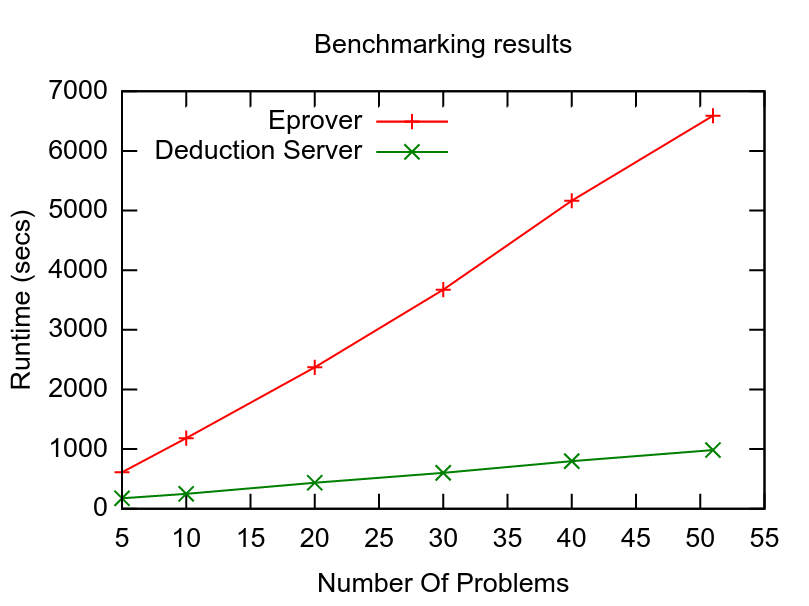
\includegraphics[width=150mm]{graphics/BenchmarkingResults.png}
  \caption{Benchmarking Results\label{benchmarking_results}}
\end{figure}

The results in Figure~\ref{benchmarking_results} shows a huge difference between the single strategy server mode and the normal eprover. That is because parsing the huge knowledge base takes large amount of time which is done in the normal eprover once for each problem. In the single strategy server mode the huge axiom set is parsed only once and kept in the server's memory and multiple queries ran against this axiom set. Therefor the per-processing time of each problem in the single strategy server mode is amortized over multiple runs.
